\createTitlePage{فصل دوم}{درک صحنه}
\subsection{درک صحنه}
درک صحنه یکی از چالش‌های اساسی در زمینه بینایی ماشین است که روش‌های مختلفی برای دست‌یابی به آن ارائه شده است. با وجود تعدد پژوهش‌های موجود در این مورد، ارائه تعریف جامع و شامل برای این مفهوم کاری بسیار دشوار است. عموما این مفهوم، بسته به مورد کاربرد و هدف پژوهش، به استخراج مجموعه مشخصی از اطلاعات در مورد صحنه که برای پژوهش، کافی و مفید باشد محدود می‌شود. به همین دلیل، مجموعه اطلاعات مطلوب از تصویر که باید استخراج شود در هر پژوهش به طور خاص تعریف می‌شود.
\\
درک صحنه در زمینه تولید خودکار شرح بر تصاویر، به طور عام شامل موارد زیر می‌شود:
\begin{enumerate}
\item تشخیص اجسام موجود در صحنه و دسته‌بندی آن‌ها (مانند توپ، تلویزیون)
\item تشخیص ارتباط مکانی بین اجسام موجود در صحنه (مانند پشت، بالا)
\item دسته‌بندی محیط (مانند جنگل، دریا)
\item دسته‌بندی فعالیت به تصویر کشیده شده (مانند راه‌رفتن، خوابیدن)
\end{enumerate}

%%%%%%%%%%%%%%%%%%%%%%%%%%%%%%%%%%%%%%%%%
\subsection{روش‌های مختلف موجود}
فعالیت‌های متعددی برای تشخیص هر یک از موارد بالا انجام شده است. به طور عام می‌توان روش‌های مورد استفاده در استخراج اطلاعات مطلوب صحنه را در زمینه تولید خودکار شرح بر تصاویر به دو دسته عمده زیر تقسیم‌بندی نمود:

\begin{enumerate}
\item استفاده از مدل‌های گرافی احتمالی\enfootnote{Probabilistic Graphical Models (PGMs)} \\

در این دسته از روش‌ها، با استفاده از مدل‌های گرافی احتمالی در مورد حضور یا عدم حضور اجسام مختلف در صحنه و رابطه بین اجسام موجود استنتاج نمود. همین‌طور فرایند‌هایی مانند قطعه‌بندی تصویر\enfootnote{Image Segmentation}
در این روش‌ها با استفاده از مدل‌های گرافی احتمالی انجام می‌شوند. به عنوان نمونه، در مقاله
\cite{fidler2013sentence}
 یک مدل میدان تصادفی شرطی\enfootnote{Conditional Random Field (CRF) }
  برای تجزیه معنایی\enfootnote{Semantic Parsin
  g} تصویر ارائه شده است که با استفاده از آن می­‌توان در مورد حضور یا عدم حضور اجسام مختلف به طور توام در صحنه تصمیم­گیری کرد.
\item استفاده از شبکه‌های عصبی کانولوشنی عمیق
در این دسته از روش‌ها، با استفاده از شبکه‌های عصبی کانولوشنی عمیق، پس از قطعه‌بندی تصاویر، اقدام به تفکیک اجسام مختلف در صحنه و برچسب‌گذاری هر جسم، بسته به یادگیری انجام شده، می‌شود. به عنوان نمونه در مقاله
\cite{karpathy2015deep}
 یک شبکه عصبی کانولوشنی عمیق معرفی شده است که قادر به برچسب‌گذاری اجسام مختلف در صحنه است. برچسب‌های مورد استفاده در این پژوهش، عبارات مختلف موجود در جملات توصیف‌گر هر تصویر در مجموعه‌دادگان هستند.

\end{enumerate}

نمونه‌های متعددی از این دست پژوهش‌ها، در هر دسته، انجام شده است که در ادامه چند مورد از آن‌ها بررسی خواهد شد.

%%%%%%%%%%%%%%%%%%%%%%%%%%%%%%%%%%%%%%%%%
\subsection{روش‌های مبتنی بر مدل‌های گرافی احتمالی}

همان‌طور که قبلا ذکر شد، روش‌های مبتنی بر استفاده از مدل‌های گرافی احتمالی، از جمله پرکاربردترین روش‌ها در مرحله درک صحنه در زمینه تولید خودکار شرح بر تصاویر هستند. این روش‌ها با استفاده از نظریه گراف، آمار و احتمالات اقدام به ارائه یک توزیع احتمالی برای پارامتر مورد بررسی، با توجه به داده‌های موجود در مجموعه آموزشی می‌کنند. مدل‌های استاندارد مختلفی در پژوهش‌ها مورد استفاده قرار می‌گیرند که تعدادی از آن‌ها به عنوان نمونه در این بخش مورد بررسی قرار خواهند گرفت.
\subsubsection[استفاده از مدل میدان تصادفی مارکف]{استفاده از مدل میدان تصادفی مارکف\enfootnote{Markov Random Field (MRF)}}
مقاله
\cite{Farhadi2010every}
با استفاده از یک مدل ساده میدان تصادفی مارکف، فرایند درک صحنه را انجام می‌دهد و با استفاده از همین مدل، اقدام به تولید جملات توصیف‌گر تصویر می‌نماید. در این فصل به بررسی فرایند درک صحنه در این مقاله می‌پردازیم و بررسی فرایند تولید جمله را به فصل بعدی موکول می‌نماییم.
\\
درک صحنه در این پژوهش محدود به ارتباط بین سه مفهوم در هر تصویر شده است؛ به این معنی که به ازای هر تصویر، یک سه‌تایی «جسم، فعالیت، صحنه»\enfootnote{<Object, Activity, Scene>}
ایجاد می‌شود که بیان‌کننده اطلاعات مطلوب موجود در تصویر است. میدان\enfootnote{Field} «جسم»، دربر دارنده‌ برچسب حاصل از دسته‌بندی اجسام موجود در صحنه، میدان «فعالیت»، دربر دارنده اطلاعات مربوط به فعالیت در حال انجام و میدان «صحنه» دربردارنده اطلاعات مربوط به محیط تصویر هستند. به فضای سه‌تایی‌های ایجاد شده برای اطلاعات مطلوب در درک صحنه، فضای معنا\enfootnote{Meaning Space} می‌گویند.
\\
شکل
\ref{fig:F2010EF1}
نمایی از نگاشت اطلاعات از فضای تصاویر و جملات به فضای معنایی، نمایش می‌دهد. همان‌طور که در شکل مشخص است، به ازای هر تصویر، یک سه‌تایی معنایی ایجاد می‌شود. همین‌طور به ازای هر جمله در فضای جملات، یک سه‌تایی ایجاد می‌شود به‌طوری‌که جملات و تصاویر متناظرشان، به یک سه‌تایی یکسان، نگاشت شوند. همان‌طور که مشخص است، با داشتن نگاشت‌هایی  که خواص مذکور را داشته‌باشند، می‌توان با استفاده از سه‌تایی‌های فضای معنا، تصاویر را مدیریت کرد.

\begin{figure}[h]
\center
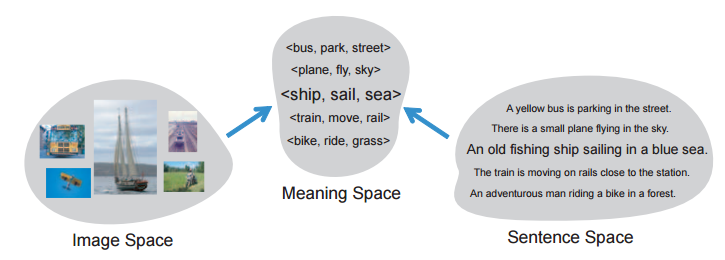
\includegraphics[scale=0.7]{./Imgs/farhadi2010every_fig1.png}
\caption{
نگاشت تصویر به فضای معنایی. فضای معنایی شامل اطلاعات مطلوب برای استخراج در فرایند درک صحنه است. به ازای هر تصویر، یک سه‌تایی ایجاد می‌شود\cite{Farhadi2010every.}
}
\label{fig:F2010EF1}
\end{figure}

مدل میدان تصادفی مارکف مورد استفاده در این پژوهش، یک مدل کوچک و ساده، شامل ۳ گره است. شکل \ref{fig:F2010EF2}
طرح‌واره‌ای از مدل میدان تصادفی مارکف مورد استفاده در این پژوهش را نمایش می‌دهد. همان‌طور که در شکل مشخص است،  به ازای هر کدام از میدان‌های تعریف شده در فضای معنایی، یک گره در این مدل وجود دارد. مقادیر مختلف در هر گره، برابر است با مقادیر مختلف موجود در میدان متناظر، در فضای معنا که با توجه به داده‌های مجموعه‌‌ ‌آموزشی مشخص می‌شوند. همین‌طور به ازای هر دو گره موجود در این مدل، یک یال بیان‌کننده ارتباط بین دو میدان در فضای معنایی وجود دارد.

برای استنتاج در این مدل، لازم است ابتدا فاکتور‌های مورد استفاده در مدل را شناخته و مقادیر آن‌ها را مشخص نماییم. در مدل پیشنهادی، دو نوع فاکتور تعریف شده است:

\begin{enumerate}
\item فاکتورهای گره\\
این فاکتورها، برای مشخص کردن میزان شباهت مقادیر مختلف گره با تصویر ورودی، تعریف شده‌‌اند. ویژگی‌‌های مورد استفاده برای مقداردهی این فاکتورها، شامل موارد زیر هستند:
\begin{enumerate}
	\item	 استفاده از آشکارکننده‌های\enfootnote{Detector}
	فلزنسوالب\enfootnote{Felzenszwaalb}، 
	به منظور محاسبه امتیاز اطمینان\enfootnote{Confidence Score} برای هر دسته از اجسام موجود در مجموعه‌داده\cite{felzenszwalb2008discriminatively}.\\
	پس از محاسبه امتیاز اطمینان همه دسته‌های موجود، دسته‌ای که بیشترین امتیاز را دارد می‌تواند به عنوان دسته‌ منتخب در میدان متناظر گره، انتخاب شود. در فرایند مقداردهی این ویژگی، قبل از انجام محاسبات، اطمینان حاصل می‌شود که از هر دسته موجود، حداقل یک تصویر در مجموعه‌داده وجود داشته باشد.
	\item استفاده از پاسخ دسته‌بندی‌کننده دیوالا\enfootnote{divvala}، ارائه شده در مقاله\cite{divvala2009empirical}
	\item استفاده از دسته‌بندی‌کننده مبتنی بر گیست\cite{Gist-based classification response}
\end{enumerate}

\begin{figure}[h]
\center
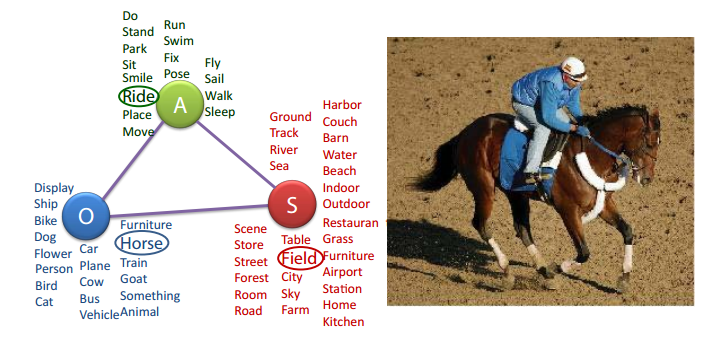
\includegraphics[scale=0.7]{./Imgs/farhadi2010every_fig2.png}
\caption{
طرح‌واره مدل میدان تصادفی مارکف ارائه شده در پژوهش \cite{Farhadi2010every} که شامل ۳ گره است. در این مدل، به ازای هر میدان از فضای معنا، یک گره وجود دارد و بین هر سه گره‌، به طور دو به دو، یک یال موجود است\cite{Farhadi2010every}.
}
\label{fig:F2010EF2}
\end{figure}

بر اساس مقادیر محاسبه شده برای ویژگی‌های بالا و با استفاده از الگوریتم ماشین بردار پشتیبان\enfootnote{Support Vector Machine (SVM)}، یک دسته‌بندی برای هر گره ارائه می‌شود که بیان‌کننده دسته‌ویژگی‌های مربوط به مقادیر مختلف گره است. با استفاده از این دسته‌بندی، با ورود هر تصویر، می‌توان برای هر مقدار در هر گره، یک امتیاز شباهت محاسبه نمود. استفاده از الگوریتم یافتن نزدیک‌ترین همسایه‌های موجود برای هر تصویر ورودی، بر اساس امتیاز شباهت محاسبه‌شده و میانگین‌گیری روی همسایه‌های استخراج شده، معیار خوبی از تخمین مقدار هر گره، به ازای هر تصویر ورودی ایجاد می‌کند. به این ترتیب، با ورود هر تصویر می‌توان برای هر کدام از گره‌های موجود در مدل، یک مقدار محتمل مشخص نمود. سه‌تایی شامل مقادیر محتمل بدست‌آمده در هر گره، سه‌تایی متناظر تصویر ورودی در فضای معنا را مشخص می‌کند.
\item فاکتورِ یال\\
این فاکتور، برای مشخص کردن میزان ارتباط مقادیر مختلف دو گره با یکدیگر در تصویر ورودی مورد استفاده قرار می‌گیرند.
\end{enumerate}

%%%%%%%%%%%%%%%%%%%%%%%%%%%%%%%%%%%%%%%%%
\subsubsection[استفاده از مدل میدان تصادفی شرطی]{استفاده از مدل میدان تصادفی شرطی\enfootnote{Conditional Random Field (CRF)}}
در این پژوهش، مساله درک صحنه در قالب یک مساله استنتاج با استفاده از مدل میدان تصادفی شرطی بیان شده است. مدل میدان تصادفی شرطی، یکی از پرکاربردترین مدل‌های گرافی احتمالی در زمینه درک صحنه است که پژوهش‌های متعددی از آن به عنوان مدل اصلی در درک صحنه استفاده کرده‌اند. به عنوان نمونه، در مقاله‌های 
\cite{Lin_2013_ICCV}
و
\cite{ladicky2010and}
از مدل میدان تصادفی شرطی به منظور توصیف صحنه استفاده شده است.\\

 پژوهش \cite{Lin_2013_ICCV} سعی در توصیف اجسام سه‌بعدی با استفاده از قطعه‌بندی تصاویر دوبعدی، هندسه سه‌بعدی و روابط بین صحنه و اجسام موجود، دارد. در این پژوهش، پس از استخراج ویژگی‌ها و اطلاعات بدست‌آمده از منابع مختلف، عمل استنتاج توسط یک مدل تصادفی شرطی انجام می‌شود که منجر به نگاشت تصویر ورودی به فضای معنایی می‌شود. همین‌طور در پژوهش \cite{ladicky2010and}، یک چارچوب کاری\enfootnote{Framework} احتمالی برای استنتاج درباره نواحی مختلف تصویر، اجسام موجود و ویژگی‌های مختلف آن‌ها مانند دسته‌بندی، موقعیت مکانی و ابعاد، مبتنی بر مدل میدان تصادفی شرطی، ارائه شده است. با توجه به وسعت و تعدد فعالیت‌های انجام شده، در این بخش، مرحله درک صحنه یک پژوهش انجام شده در زمینه تولید خودکار شرح بر تصاویر را مورد بررسی قرار می‌دهیم. لازم به ذکر است، مرحله تولید جملات توصیف‌کننده پژوهش مورد بحث، در فصل تولید جملات زبان طبیعی مورد بررسی قرار خواهد گرفت.
\\
در پژوهش\cite{fidler2013sentence}
از مدل میدان تصادفی شرطی برای توصیف صحنه و اجسام موجود در آن استفاده شده است. میدان‌های تصادفی در این مدل، شامل متغیرهای زیر هستند:
\begin{enumerate}
\item  متغیرهای تصادفی بیان‌کننده برچسب دسته متناظر قطعات مختلف هر تصویر به شیوه سلسله مراتبی دارای دو سطح
\item متغیرهای تصادفی باینری بیان‌کننده صحت دسته‌ تشخیص داده‌شده برای هر جسم
\end{enumerate}

شکل
\ref{fig:F2013SF1}
 طرح‌واره مدل سلسله‌مراتبی ارائه شده در پژوهش \cite{fidler2013sentence} را نمایش می‌دهد. همان‌طور که مشاهده می‌شود این مدل از دو سطح انتزاع، یکی برای برچسب قطعات مختلف تصویر و دیگری برای حضور یا عدم حضور هر دسته از اجسام در تصویر، تشکیل شده است.

\begin{figure}[h]
\center
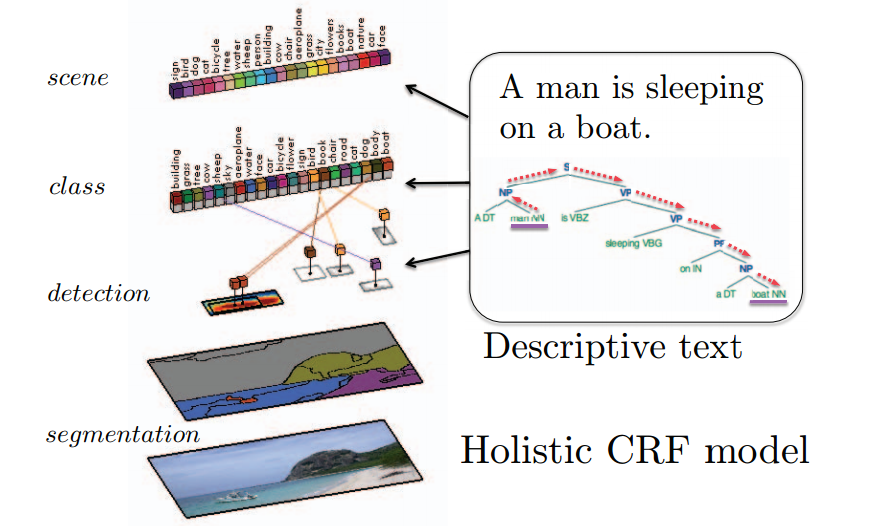
\includegraphics[scale=0.5]{./Imgs/fidler2013sentence_f1.png}
\caption{طرح‌واره مدل سلسله مراتبی مبتنی بر میدان تصادفی شرطی که بر اساس اطلاعات بصری و اطلاعات جملات توصیف‌کننده شرح محتمل تصویر را تولید می‌نماید\cite{fidler2013sentence}.}
\label{fig:F2013SF1}
\end{figure}

دو دسته متغیر تصادفی مختلف، که هر یک نماینده متغیرهای تصادفی موجود در یکی از این سطوح انتزاع هستند، تعریف شده‌اند؛ 
متغیرهای تصادفی $X_i \in {1, \cdots,C}$ بیان‌کننده دسته قطعه $i$ام از سطح پایین سلسله مراتب و متغیرهای تصادفی $Y_j \in {1, \cdots,C}$ بیان‌کننده دسته قطعه $j$ام از سطح بالای سلسله مراتب.
به علاوه، دو دسته متغیر تصادفی دیگر به نام‌های $b_l$ و $z_k$ به ترتیب برای نمایش حضور یا عدم حضور یک تشخیص کاندید\enfootnote{Candidate Detection} و حضور یا عدم حضور جسم با دسته $k$ در تصویر، تعریف شده‌اند. با توجه به متغیرهای تعریف شده، مدل کلی میدان تصادفی شرطی را می‌توان معادل رابطه\ref{eq:crffidler} تعریف کرد. در این رابطه $\Psi_\alpha^{type}(a_\alpha)$ نماینده تابع پتانسیل تعریف شده روی متغیرهای مختلف است. با این تعریف، یافتن تخمین \lr{MAP}\enfootnote{MAP Estimation}، منجر به یافتن پاسخ مورد نظر می‌شود.
در ادامه، توابع پتانسیل مختلف که در این پژوهش تعریف شده‌اند، ارائه خواهد شد. لازم به ذکر است در تمام این موارد، برای سهولت، توابع پتانسیل به شکل لگاریتمی تعریف شده‌اند.
\begin{equation}
P(X,Y,b,z) = \frac{1}{Z} \mathlarger{\mathlarger{\Pi}}_{type} \mathlarger{\mathlarger{\Pi}}_\alpha \Psi_\alpha^{type}(a_\alpha)
\label{eq:crffidler}
\end{equation}

توابع پتانسیل مختلف تعریف شده در این پژوهش عبارتند از:

\begin{enumerate}
\item پتانسیل قطعه‌بندی یگانی\enfootnote{Unary Segmentation Potential}\\
پتانسیل قطعه‌بندی یگانی در هر قطعه و هر ابرقطعه\enfootnote{Supersegment} از تصویر، با استفاده از میانگین‌گیری روی امتیاز افزایش تکستون\enfootnote{Texton Boost} که در پژوهش \cite{ladicky2010graph} ارائه شده است، انجام می‌شود.
\item انطباق بین متغیرهای دو سطح انتزاع با یک‌دیگر\\
یک مقدار جریمه به ازای دسته‌های مخالف بین دو سطح در نظر گرفته‌ می‌شود تا در حد امکان، دسته‌های منتخب از بین سطوح مختلف، با یک‌دیگر انطباق داشته باشند. پتانسیل تعریف شده در این بخش معادل رابطه\ref{eq:phiijf} 
تعریف می‌شود.
	\begin{equation}
		\phi_{ij}(X_i, Y_j)=
			\left\{
				\begin{array}{ll}
					- \gamma		&	X_i \neq Y_j \\
					0			&	X_i	=	Y_j
				\end{array}							
			\right.
		\label{eq:phiijf}
	\end{equation}
در رابطه\ref{eq:phiijf}، پارامتر $\gamma$ در فرآیند یادگیری که منجر به بهینه‌سازی پارامترهای مختلف مدل می‌شود، به‌دست می‌آید.
\item پتانسیل انطباق تصویر و دسته جسم\\
برای اندازه‌گیری میزان انطباق هر کدام از دسته‌های موجود برای اجسام با تصویر ورودی، از معیار انطباق ارائه شده در پژوهش\cite{felzenszwalb2010object}
 توسط فلزنسوالب که به روش دی پی ام\enfootnote{DPM} مشهور است، استفاده شده است. برای کاهش تعداد پارامترها و افزایش کارایی مدل استفاده شده، برای هر تصویر حداکثر ۳ دسته جسم، به عنوان دسته‌های منتخب کاندید، در نظر گرفته می‌شوند.
\end{enumerate}


%%%%%%%%%%%%%%%%%%%%%%%%%%%%%%%%%%%%%%%%%
\subsubsection{استفاده از سایر مدل‌های گرافی احتمالی}
در بین پژوهش‌های موجود در زمینه درک صحنه با استفاده از روش‌های احتمالاتی، علاوه بر مدل‌های استاندارد، از مدل‌های مولد دیگر در پژوهش‌های متعددی استفاده شده است. در ادامه این بخش، به بررسی چند‌ نمونه از این مدل‌ها خواهیم پرداخت.

\begin{enumerate}
\item دسته‌بندی تصاویر بر اساس صحنه و اجسام موجود به طور توام\cite{li2007and}

مدل استفاده شده در این پژوهش، از تصاویر در سطح صحنه و سطح اجسام استفاده کرده و با یکپارچه‌سازی و تجمیع اطلاعات موجود در این دو سطح، اقدام به دسته‌بندی تصویر می‌نماید. شکل\ref{fig:l2007af1} 
مدل استفاده شده در این پژوهش را به منظور یکپارچه‌سازی و تجمیع اطلاعات حاصل از تحلیل صحنه و تشخیص اجسام موجود در آن، ارائه می‌دهد.


\begin{figure}[H]
\center
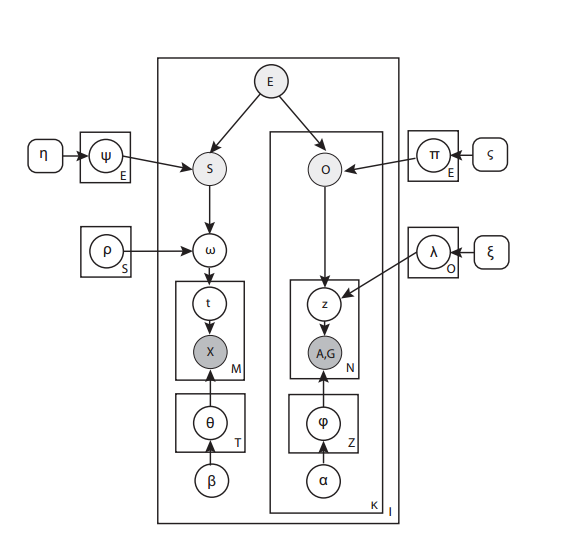
\includegraphics[scale=0.5]{./Imgs/li2007and_model.png}
\caption{مدل استفاده شده به منظور تجمیع اطلاعات صحنه و اجسام موجود در آن به منظور دسته‌بندی تصاویر\cite{li2007and}}
\label{fig:l2007af1}
\end{figure}

یکی از اهدافی که در این پژوهش دنبال می‌شود، برچسب‌گذاری معنایی\enfootnote{Semantic Labelling} تمام پیکسل‌های موجود در تصویر است. به همین منظور، تمام تصاویر مورد استفاده، به نواحی $10 * 10$ تقسیم شده و مورد استفاده قرار می‌گیرند. برای بررسی بهتر مدل، ابتدا متغیرهای تصادفی مورد استفاده را تعریف کرده و سپس به بررسی روند یادگیری و استنتاج مدل می‌پردازیم.
\\
متغیر تصادفی $X$ که حاوی اطلاعاتی مبتنی بر حضور یا عدم حضور دسته‌های مختلف صحنه است، در بخش تشخیص صحنه به‌کار می‌رود. اطلاعات این متغیر با استفاده از توصیف‌کننده سیفت\enfootnote{SIFT Descriptor} و به ازای هر ناحیه از تصویر، به‌دست می‌آید. برای بخش تشخیص اجسام موجود در صحنه، از دو منبع اطلاعاتی مختلف استفاده می‌شود. اطلاعات مربوط به حضور یا عدم حضور دسته‌های مختلف اجسام در متغیر تصادفی $A$ و اطلاعات مربوط به شکل کلی آن‌ها در متغیر تصادفی $G$ نمایش داده‌ می‌شود.
\\
هر گره از مدل ارائه شده، نماینده یک متغیر تصادفی است. گره‌هایی که با رنگ تیره مشخص شده‌اند، نماینده متغیرهایی هستند که در فرایند آموزش دیده می‌شوند و بقیه متغیرها، متغیرهای مخفی\enfootnote{Latent} هستند. گره‌های خاکستری روشن‌تر، متغیرهایی هستند که فقط در فرایند آموزش دیده‌ می‌شوند در حالی‌که متغیرهای تیره‌تر در هر دو فرایند آموزش و آزمون مشاهده می‌شوند.
\\
متغیر تصادفی $E$، نماینده یک دسته‌ از رخداد
\enfootnote{Event}
های ممکن است. توزیع احتمال اولیه این متغیر  تصادفی، یک توزیع یکنواخت فرض شده است که به هر تصویر ورودی، بر اساس همین توزیع، یک مقدار خاص از این متغیر تصادفی اختصاص داده می‌شود. با دانستن دسته رخداد موجود در تصویر، یک تصویر صحنه\enfootnote{Scene Image} متناظر با تصویر ورودی تولید می‌شود. با فرض وجود $S$ دسته صحنه مختلف در مجموعه‌داده، به هر تصویر، تنها یک دسته صحنه اختصاص داده می‌شود. روند اختصاص دسته صحنه به تصویر مطابق زیر است:
\begin{itemize}
\item[*]
ابتدا یک دسته اولیه مطابق با توزیع احتمال شرطی 
$P(S|E, \psi)$
به تصویر اختصاص داده می‌شود. $\psi$ یک پارامتر چندجمله‌ای
\enfootnote{Multinomial}
 حاکم بر توزیع احتمالاتی $S$ به شرط داشتن $E$ است. به علاوه، $\psi$ یک ماتریس به ابعاد $E * S$ و پارامتر $\eta$ یک بردار $S$ بعدی در نقش مقدار اولیه دیریکله
\enfootnote{Dirichlet prior}
 برای پارمتر $\psi$ است.
\item[*]
در قدم بعدی با داشتن مقدار $S$، پارامترهای $\omega$ را بر اساس احتمال 
$P(\omega|S, \rho)$
تولید می‌کنیم. از آن‌جا که $\omega$ پارامتر چندجمله‌ای گره‌های مخفی $t$ هستند، باید مجموع همه آن‌ها برابر با یک باشد. به علاوه، $\rho$ یک ماتریس به ابعاد $S * T$ و مقدار اولیه دیریکله برای پارامتر $\omega$ است که در آن $T$ تعداد کل $t$ها است.
\item[*] 
برای تولید هر یک از $M$ ناحیه تصویر (مقادیر متغیر تصادفی $X$) به شکل زیر عملی می‌کنیم:
\begin{itemize}
\item[-]
یک مقدار $t$ از توزیع احتمال $Mult(\omega)$ تولید می‌شود که مشخص‌کننده موضوعی\enfootnote{Topic} است که این ناحیه از تصویر مطابق با آن تولید شده است.
\item[-]
متغیر تصادفی $X$ از توزیع احتمالی 
$P(X|t,\theta)$ تولید می‌شود.
$\theta$ یک ماتریس به ابعاد
$T * V_s$ است که در آن
$V_s$ تعداد کلمات موجود در پایگاه داده مربوط به صحنه $s$  است.
به علاوه، $\theta$ یک پارامتر چندجمله‌ای برای $X$ است و $\beta$ مقدار اولیه دیریکله برای $\theta$.
\end{itemize}
\end{itemize}

همانند فرایندی که طی آن، تصویر صحنه به تصویر ورودی اختصاص داده می‌شود، فرایندی وجود دارد که طی آن تصویر اجسام\enfootnote{Object Image} به تصویر ورودی اختصاص داده می‌شود. بر خلاف صحنه، هر تصویر می‌تواند بیش از یک جسم داشته باشد. تعداد کل اجسام موجود در یک تصویر را با $K$ و تعداد کل دسته‌های موجود برای اجسام در مجموعه‌داده را با $O$ نمایش می‌دهیم. فرایند زیر برای هر یک از $K$ جسم موجود در تصویر اجرا می‌شود:

\begin{itemize}
\item[*]
ابتدا یک دسته جسم با توزیع احتمالی  
$P(O|E, \pi)$
به تصویر اختصاص داده می‌شود که در آن، $\pi$ یک ماتریس به ابعاد $E * O$ و $\zeta$ یک بردار به طول $O$ و مقدار اولیه دیریکله پارامتر $\pi$ است.
\item[*]
سپس با داشتن $O$ می‌توان تمام نواحی $A$ و $G$ مرتبط با دسته جسم را تولید نمود. فرایند تولید این نواحی به شکل زیر است:
	\begin{itemize}
	\item[-]
	متغیر تصادفی مخفی $z$ که مشخص کننده موضوع است، از توزیع احتمالی $Mutl(\lambda,|O)$ تولید می‌شود. متغیر $\lambda$ یک ماتریس به ابعاد $O * Z$ است که در آن  $Z$ تعداد کل مقادیر مختلف متغیر $z$ است. به علاوه $\xi$ مقدار اولیه دیریکله برای پارامتر $\lambda$ است.
	\item[-]
	نواحی مطلوب از توزیع احتمال $P(A,G|t, \phi)$ تولید می‌شوند که در آن، $\phi$ یک ماتریس به ابعاد $Z * V_o$ است. $V_o$ تعداد کل کلمات موجود در مجموعه‌داده، به ازای نواحی $A$ و $G$ است. پارامتر $\alpha$ مقدار اولیه دیریکله برای پارامتر $\phi$
است. 	
	\end{itemize}
\end{itemize}

با توجه به متغیرهای تصادفی توضیح داده شده در بالا، توزیع احتمالی توام کل سیستم را می‌توان مطابق با رابطه 
\ref{eq:liJP}
تعریف کرد.

\begin{equation}
\label{eq:liJP}\begin{split}
P(E,S,O,X,A,G,t,z,\omega |\rho ,\phi ,\lambda ,\psi ,\pi \theta) &= P(E)\cdot P(S|E,\psi)\cdot P(\omega|S,\rho) \\ 
&\cdot \mathlarger{\mathlarger{\Pi}}_{m=1}^M P(X_m|t_m,\theta)\cdot P(t_m|\omega) \\
&\cdot \mathlarger{\mathlarger{\Pi}}_{k=1}^K P(O_k|E,\pi)\\
&\cdot \mathlarger{\mathlarger{\Pi}}_{n=1}^N P(A_n,G_n|z_n,\phi)\cdot P(z_n|\lambda,O_k)
\end{split}
\end{equation}

به علاوه، با توجه به توضیحات ارائه شده در بالا، هر کدام از عبارات موجود در رابطه \ref{eq:liJP} را می‌توان با عبارات معادل آن‌ها که در روابط
\ref{eq:liSF}
تا
\ref{eq:liSL}
آمده، جایگزین نمود.

\begin{align}
&P(S|E,\psi) = Mult(S|E,\psi)
\label{eq:liSF}
\\
&P(\omega|S,\rho) = Dir(\omega|\rho_{j.}), S = j
\\
&P(t_m|\omega) = Mult(t_m|\omega)
\\
&P(X_m|t_m,\theta) = P(X_m|\theta_{j.}), t_m = j
\\
&P(O_k|E,\pi) = Mult(O_k|E,\pi)
\\
&P(z_n|\lambda,O_k) = Mult(z_n|\lambda,O_k)
\\
&P(A_n,G_n|z_n,\phi) = P(A_n,G_n|\phi_{j.}), z_n = j
\label{eq:liSL}
\end{align}

درک صحنه در این پژوهش، محدود به استخراج سه دسته اطلاعات زیر از تصویر است:

\begin{enumerate}
\item رخدادی که در تصویر به نمایش گذاشته شده است.
\item صحنه‌ای که تصویر در آن ایجاد شده است.
\item اجسامی که در تصویر حضور دارند.
\end{enumerate}

با توجه به این محدودیت و با در نظر گرفتن مدل ارائه شده، استفاده از تخمین بیشینه احتمال\enfootnote{Maximum Likelihood}، می‌تواند برای استخراج اطلاعات مطلوب مفید باشد. از همین رو، تخمین بیشینه احتمال، در سه سطح مختلف (هر سطح برای یک دسته از اطلاعات مطلوب) اعمال می‌شود. در سطح اجسام، احتمال رخداد تصویر ورودی به شرط اجسام موجود مطابق با رابطه 
\ref{eq:liPIO}، احتمال رخداد تصویر ورودی به شرط صحنه، مطابق با رابطه 
\ref{eq:liPIS}
و احتمال رخداد تصویر ورودی به شرط دسته رخداد به نمایش‌گذاشته شده در تصویر، مطابق با رابطه 
\ref{eq:liPIE}
محاسبه می‌شوند.
\begin{align}
&P(I|O) = \ML{\Pi}_{n=1}^N \ML{\Sigma}_j P(A_n,G_n|z_j,O) P(z_j|O)
\label{eq:liPIO}
\\
&P(I|S,\rho,\theta) = \int P(\omega|\rho,S)(\ML{\Pi}_{m=1}^M \ML{\Sigma}_{t_m} P(t_m|\omega) P(X_m|t_m, \theta) ) d\omega
\label{eq:liPIS}
\\
&P(I|E) \propto \ML{\Sigma}_j P(I|O_j) P(O_j|E) P(I|S) P(S|E)
\label{eq:liPIE}
\end{align}

فرایند یادگیری این مدل، شامل یافتن بهترین مقادیر برای پارامترهای 
$\{\psi,\rho,\pi,\lambda,\theta,\beta\}$
است.
این فرایند برای سه پارامتر 
$\{\psi,\rho,\theta\}$ 
با استفاده از روش انتقال پیام متغیر\enfootnote{Variational Message Passing} و برای سه پارامتر
$\{\pi,\lambda,\beta\}$
با استفاده از نمونه‌برداری گیبس\enfootnote{Gibbs Sampling} انجام می‌شود.
\\
آزمایشات انجام شده در این پژوهش، بر روی یک مجموعه‌داده شامل تصاویر از ۸ دسته ورزشی مختلف که در هر دسته، بین 137 تا 250 تصویر مختلف وجود دارد، انجام شده‌اند. از جمله چالش‌های موجود در این مجموعه‌داده می‌توان به وجود زمینه‌های متنوع و پیچیده در تصاویر، تنوع دسته‌های مختلف اجسام موجود، تنوع اندازه اجسام موجود از یک دسته، تنوع حالت اجسام، تنوع تعداد نمونه‌های یک جسم در یک تصویر و کوچک بودن بیش از اندازه ابعاد اجسام در تصویر اشاره کرد. شکل
\ref{fig:lid}
نمونه‌ای از تصاویر موجود در این مجموعه‌داده را نمایش می‌دهد.

\begin{figure}[H]
\center
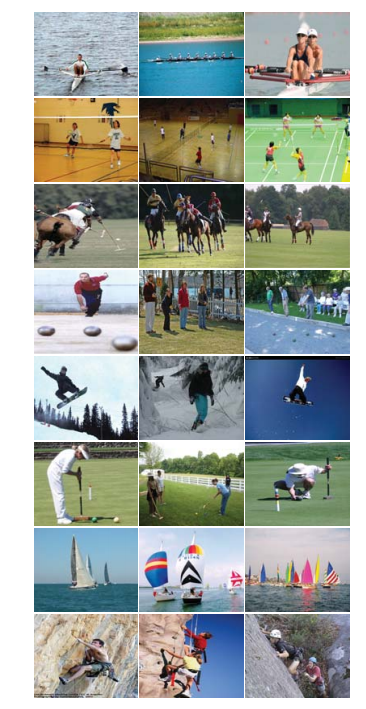
\includegraphics[scale=0.95]{./Imgs/li2007and_dataset.png}
\caption{نمونه تصاویر موجود در مجموعه‌داده مورد استفاده. \cite{li2007and}}
\label{fig:lid}
\end{figure}

استفاده از مدل کامل ارائه شده در این پژوهش، منجر به تشخیص صحیح 73.4\% از تصاویر شده است. شکل
\ref{fig:liCM}
 ماتریس درهم‌ریختگی
\enfootnote{Confusion Matrix}
 مربوط به این مدل را نمایش می‌دهد. همان‌طور که در این ماتریس مشخص است، کمترین نرخ تشخیص در بین دسته‌های ورزشی موجود در این مدل، 52\% و بیشترین نرخ تشخیص 92\% است.

\begin{figure}[H]
\center
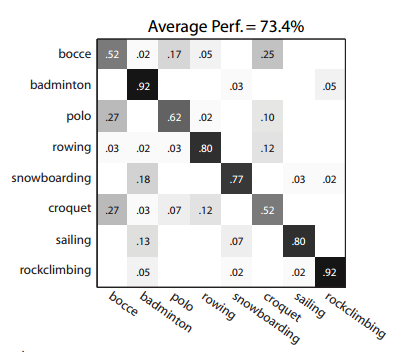
\includegraphics[scale=0.8]{./Imgs/li2007and_confmat.png}
\caption{ماتریس درهم‌ریختگی مدل کامل ارائه شده برای مجموعه‌داده شامل ۸ دسته تصویر ورزشی. \cite{li2007and}}
\label{fig:liCM}
\end{figure}

بسته به میزان استفاده از اطلاعات مختلف استخراج شده برای استنتاج، مدل‌های مختلفی به‌وجود می‌آیند که در شکل
\ref{fig:liCMP}
نتایج عملکرد هریک از این مدل‌ها با مدل‌های دیگر مقایسه شده است.
همان‌طور که در شکل \ref{fig:liCMP}
مشخص است، بهترین کارایی مربوط به مدل کامل است. در صورتی‌که در مدل، فقط از اطلاعات مربوط به صحنه استفاده شود، نتایج بدست‌آمده اگرچه با نتایج مدل کامل قابل مقایسه نیست، از نتایج مدل مبتنی بر اطلاعات جسم بهتر است.

\begin{figure}[H]
\center
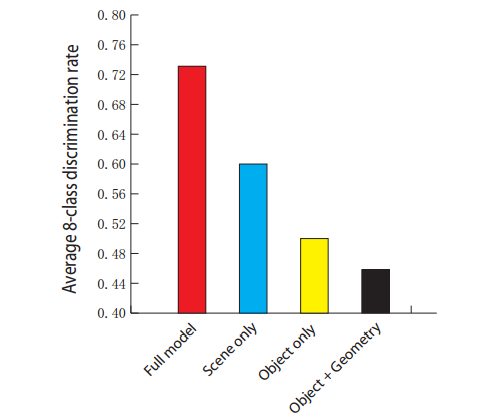
\includegraphics[scale=0.6]{./Imgs/li2007and_compar.png}
\caption{نتیجه مقایسه مدل‌های مختلف به‌وجود آمده بسته به سطح اطلاعات مورد استفاده برای استنتاج. \cite{li2007and}}
\label{fig:liCMP}
\end{figure}

شکل
\ref{fig:liR}
نتایج نهایی به‌دست آمده از مدل را نمایش می‌دهد. در این شکل، تصاویر موجود در هر سطر نماینده تصاویر موجود در یکی از دسته‌های ورزشی هستند. ستون اول برچسب به‌دست آمده از رخداد موجود در تصویر، ستون دوم برچسب‌های تشخیص داده شده مربوط به اجسام موجود، ستون سوم برچسب اختصاص داده‌شده مربوط به دسته صحنه و ستون چهارم توزیع مرتب شده اجسام به شرط رخداد را به نمایش می‌گذارند. در نمودارهای موجود در ستون چهارم، محور افقی شامل نام اجسام و محور عمودی مقدار توزیع را نمایش می‌دهد.

\begin{figure}[H]
\center
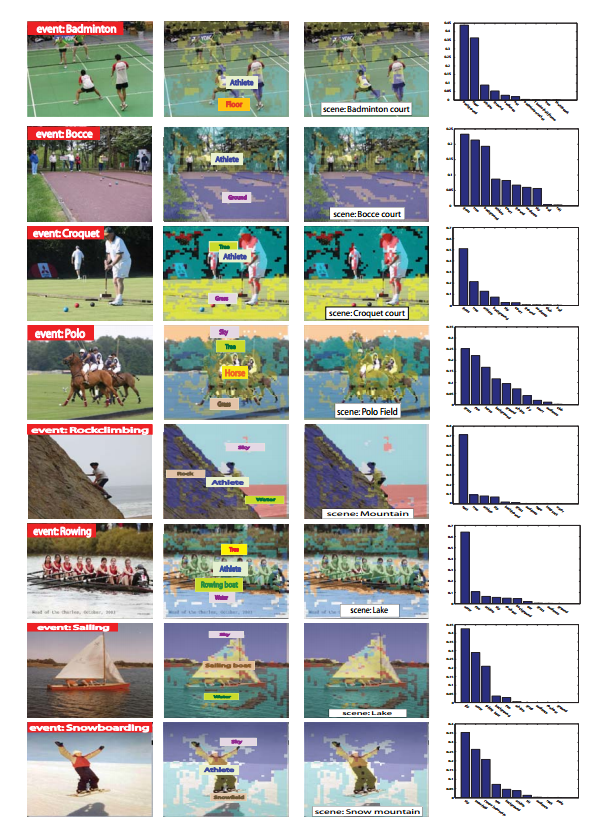
\includegraphics[scale=0.8]{./Imgs/li2007and_res1.png}
\caption{نتایج نهایی به‌دست آمده از مدل بر روی تصاویر. \cite{li2007and}}
\label{fig:liR}
\end{figure}



%%%%%%%%%%%%%%%%%%%%%%%%%%%%%%%%%%%%%%%%%%%%%%%%%%%%
\item حاشیه‌نویسی تصویر\enfootnote{Image Annotation} با استفاده از قطعه‌بندی و دسته‌بندی صحنه و اجسام موجود\cite{li2009towards}





\item درک صحنه بر اساس نواحی مختلف تصویر، اجسام موجود و روابط سه‌بعدی بین ‌آن‌ها\cite{gould2009decomposing}
\end{enumerate}

%%%%%%%%%%%%%%%%%%%%%%%%%%%%%%%%%%%%%%%%%
\subsection{روش‌های مبتنی بر شبکه‌های عصبی کانولوشنی عمیق}

علاوه بر فعالیت‌هایی که در زمینه تولید خودکار شرح بر تصاویر با رویکرد احتمالاتی انجام شده‌اند، تعداد زیادی از پژوهش‌گران تلاش می‌کنند تا با استفاده از روش‌‌های مبتنی بر شبکه‌های عصبی با این چالش روبرو شوند. در این بخش تعدادی از پژوهش‌هایی را که با استفاده از شبکه‌های عصبی سعی در درک صحنه‌های موجود در تصاویر دارند را مورد بررسی قرار می‌دهیم. شایان ذکر است، در این بخش تنها به بررسی بخشی از پژوهش‌ها که مربوط به درک صحنه است می‌پردازیم و بخش‌هایی از این پژوهش‌ها که مربوط به تولید جملات زبان طبیعی متناسب با تصویر و صحنه درک شده است را در فصل تولید جملات زبان طبیعی بررسی خواهیم نمود.
\\
یکی از مهم‌ترین عملیات‌هایی که به نحوی در تمام پژوهش‌های قبلی وجود داشت، اختصاص یک معنا به قطعه‌های مختلف یک تصویر است. این چالش، در پژوهش‌های مرتبط با تولید خودکار شرح بر تصاویر که با استفاده از روش‌های مبتنی بر شبکه‌های عصبی به دنبال حل مشکل هستند نیز مطرح است. در ابتدا به بررسی یکی از روش‌های اختصاص معنا به هر قطعه ازتصویر می‌پردازیم.

\subsubsection[اختصاص معنا به قطعه‌های مختلف تصویر]{اختصاص معنا به قطعه‌های مختلف تصویر\cite{Girshick_2014_CVPR}}
در پژوهش 
\cite{Girshick_2014_CVPR}
روشی ارائه شده است که با استفاده از یک شبکه عصبی کانولوشنی عمیق، علاوه بر این که می‌تواند یک تصویر را به شکل پایین به بالا، در قالب نواحی سلسله‌مراتبی قطعه‌بندی کند، قادر به استفاده به عنوان یک شبکه از پیش آموزش  دیده‌شده در پژوهش‌های مرتبط دیگر باشد.
\\
فرایند تشخیص اجسام در این پژوهش از سه بخش اصلی تشکیل شده است:
\begin{enumerate}
\item
طرح پیشنهاداتی برای نواحی به طور مستقل از دسته‌بندی\enfootnote{Category-independent region proposals}
\item 
یک شبکه عصبی عمیق کانولوشنی که وظیفه استخراج ویژگی برای هر ناحیه را بر عهده دارد (طول بردار ويژگی استخراج شده برای تمام نواحی یکسان است).
\item
مجموعه‌ای از ماشین‌های بردار پشتیبان خطی مخصوص هر دسته
\end{enumerate}
در ادامه به بررسی نحوه پیشنهاد نواحی و شبکه عصبی کانولوشنی عمیق مورد استفاده در ای پژوهش می‌پردازیم.

\begin{enumerate}
\item طرح پیشنهاد نواحی\\
روش‌های مختلفی برای پیشنهاد نواحی ارائه شده‌اند که در اینجا از روشی موسوم به جستجوی انتخابی\enfootnote{Selective Search} استفاده می‌شود. نسخه‌های مختلفی از این روش ارائه شده است. نسخه ارائه شده در پژوهش
\cite{uijlings2013selective}،
یکی از سریع‌ترین نسخه‌های ارائه شده است که در این بخش از همین روش استفاده می‌شود.
\\
در پژوهش 
\cite{uijlings2013selective}
دو ویژگی‌ مطرح شده است که یک جستجوی انتخابی برای ارائه نواحی معنایی تصویر باید آن‌ها را داشته باشد. ویژگی اول این است که اجسام موجود در فضا می‌توانند در هر اندازه‌ای باشند و در نتیجه نواحی ارائه شده باید بتوانند ابعاد مختلف داشته باشند. این ویژگی عموما با روش‌های سلسله‌مراتبی قابل دست‌یابی است. ویژگی دوم این است که نواحی مختلف باید براساس  ویژگی‌های مختلفی تولید شوند. در صورتی‌که یک ویژگی مثل رنگ، بافت، روشنایی یا مواردی از این دست، به عنوان تنها ویژگی برای تشخیص نواحی به کار گرفته شود، الگوریتم قادر به ارائه نواحی مناسب در شرایط مختلف نخواهد بود. بنابراین ترکیب چند معیار و ویژگی باید برای تشخیص نواحی مورد استفاده قرار بگیرد. 
\\
برای دست‌یابی به ویژگی اول، ابتدا نواحی اولیه کوچکی روی تصویر ایجاد می‌شود. سپس با اتخاذ یک روش حریصانه و تعریف یک معیار شباهت بین نواحی همسایه، ناحیه‌هایی که شباهت زیادی با یک‌دیگر دارند و همسایه هستند، با هم ترکیب شده و یک ناحیه بزرگ‌تر ساخته می‌شود. به این ترتیب یک روش سلسله‌مراتبی برای ساخت نواحی با ابعاد مختلف به‌دست ‌می‌آید.برای دست‌یابی به ویژگی دوم، از فضاهای رنگی مختلف، معیارهای شباهت مختلف و نواحی اولیه متفاوت و ترکیب پاسخ این ویژگی‌ها با هم برای ارائه نواحی و ترکیب نواحی کوچک‌تر استفاده می‌شود.

\item شبکه عصبی کانولوشنی عمیق (استخراج ویژگی‌ها)\\
در این بخش از یک شبکه عصبی کانولوشنی عمیق از پیش‌آموزش‌دیده‌ برای استخراج ویژگی ‌از هر ناحیه ارائه شده در قسمت قبل، استفاده می‌شود. بردار ویژگی استخراج شده برای هر ناحیه یک بردار شامل 4096 مولفه است که خروجی شبکه کریشفسکی\enfootnote{Krizhevsky}
آزمایش شده در چالش دسته‌بندی اجسام مسابقه  \lr{ImageNet} است. اطلاعات دقیق درباره این شبکه عصبی در پژوهش 
\cite{krizhevsky2012imagenet}
در دسترس است.

\end{enumerate}

شبکه عصبی کانولوشنی عمیق ارائه شده در این پژوهش با استفاده از یک مجموعه‌داده\enfootnote{ILSVRC 2012} آموزش دیده شده است. از این شبکه عصبی که تحت عنوان \lr{RCNN}\enfootnote{Regional Convolutional Neural Network} شناخته می‌شود می‌توان به عنوان یک شبکه از پیش‌آموزش‌دیده استفاده کرد.

\subsubsection[ناحیه‌بندی عمیق تصاویر به منظور نگاشت دوطرفه جملات و تصاویر]{ناحیه‌بندی عمیق تصاویر به منظور نگاشت دوطرفه جملات و تصاویر\cite{karpathy2014deep}}

مدل ارائه شده در این پژوهش، مدلی است که قادر به نگاشت دوطرفه تصاویر و جملات به یک‌دیگر است. شکل\ref{fig:k2014DM} طرح‌واره‌ای از این مدل را نمایش می‌دهد. ورودی مدل در سمت چپ، تصاویر و در سمت راست، جملات هستند. در این مدل، ابتدا تصاویر ورودی با استفاده از یک شبکه عصبی \lr{RCNN} تبدیل به نواحی مختلف شده و برای هر ناحیه یک بردار ویژگی 4096 بعدی استخراج می‌شود. سپس با اعمال روش خاصی روی جملات ورودی از سمت راست (که در بخش تولید جملات زبان طبیعی به بررسی آن خواهیم پرداخت) قطعات مختلف موجود در جملات نیز استخراج شده و بین هر قطعه از جمله با تمام نواحی استخراج شده از تصویر یک معیار شباهت محاسبه می‌شود و شبیه‌ترین قطعه جمله با ناحیه مربوط به خود در تصویر، جفت می‌شوند.

\begin{figure}[H]
\center
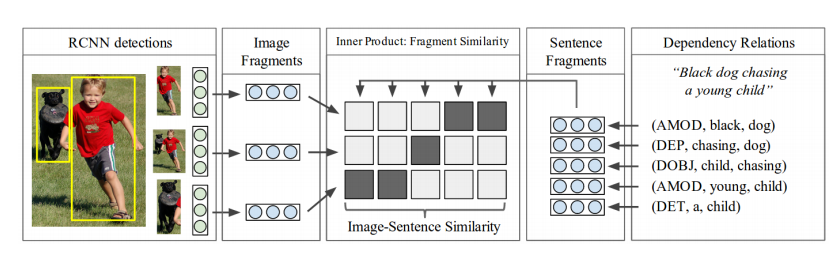
\includegraphics[scale=0.6]{./Imgs/karpathy2014deep_model.png}
\caption{مدل استفاده شده برای نگاشت دو‌طرفه تصاویر و جملات به یک‌دیگر با استفاده از شکبه‌ عصبی عمیق کانولوشنی.\cite{karpathy2014deep}}
\label{fig:k2014DM}
\end{figure}

در این پژوهش پس از ناحیه‌بندی تصویر توسط شبکه \lr{RCNN}، برای هر تصویر ۱۹ ناحیه استخراج می‌شود. این ۱۹ ناحیه در کنار تصویر اصلی، یک مجموعه شامل ۲۰ تصویر ایجاد می‌کنند که در پردازش‌های بعدی مورد استفاده قرار خواهند گرفت. در این مرحله باید تمام تصاویر موجود را با استفاده از یک نگاشت به فضای برداری ویژگی‌ها تبدیل نمود. برای این کار از رابطه\ref{eq:k2014ISV}
استفاده می‌شود. در این رابطه، $I_b$ مجموعه تمام پیکسل‌های موجود در ناحیه $b$،
$RCNN_{\theta_c}$
شبکه عصبی آموزش‌دیده است که در آن $\theta_c$ مجموعه پارامترهای بهینه موجود در شبکه است. بردار حاصل $\nu_i$ برای تصویر $i$ام، بردار نگاشت تصویر به فضای معنایی خواهد بود که محاسبه مقادیر آن مبتنی بر پیشنهاد نواحی معنایی مختلف و محاسبه ويژگی‌های مختلف روی هر ناحیه است.

\begin{equation}
\nu = W_m[RCNN_{\theta_c}(I_b)] + b_m
\label{eq:k2014ISV}
\end{equation}

از طرفی با در نظر گرفتن بردار $s_j$ به عنوان بردار حاصل از نگاشت جمله $j$ام به فضای معنایی و در نظر گرفتن ضرب داخلی به عنوان شباهت، $\nu_i^T \cdot s_j$
معیار شباهت بین یک تصویر و یک جمله را تعریف می‌کند.
با توجه به توضیحات ارائه شده، می‌توان تابع هدف را برای شبکه کلی معادل سیستم ارائه داد. دو هدف اصلی در این شبکه قابل تعریف است:
\begin{enumerate}
\item رتبه‌بندی سراسری\\
 تصاویر و جملاتی که در فرایند محاسبات شبکه عصبی بیشترین شباهت را با یک‌دیگر دارند باید در واقعیت هم بیشترین شباهت و ارتباط را داشته باشند.
\item هم‌ترازسازی ناحیه‌ای\enfootnote{Fragment Alignment}\\
نواحی استخراج شده تصویر و عبارات استخراج شده جملات که در محاسبات شبکه عصبی بیشترین شباهت را با یک‌دیگر دارند، باید در واقعیت هم بیشترین شباهت و ارتباط را داشته باشند.
\end{enumerate}

با توجه به مطالب گفته شده، می‌توان تابع هدف کلی را مطابق با رابطه\ref{eq:k2014Obj}
تعریف کرد.
در این رابطه، $\Theta$ مجموعه پارامترهای شبکه عصبی شامل 
$\{W_m,b_m,\theta_c,W_e,W_R\}$
است (پارامترهای $W_e$ و‌ $W_R$ مربوط به بخش تحلیل جمله هستند که در فصل مربوطه بررسی خواهند شد). $C_F$ تابع هدف هم‌ترازسازی ناحیه‌ای، $C_G$ تابع هدف سراسری، $\alpha$ و $\beta$ دو ابرپارامتر\enfootnote{Hyperparameter} (با آزمون و خطا تعیین می‌شوند) و $||\Theta||_2^2$ یک عبارت تنظیم‌کننده\enfootnote{Regularization Term} هستند.

\begin{equation}
C(\Theta) = C_F(\Theta) + \beta C_G(\Theta) + \alpha ||\Theta||_2^2
\label{eq:k2014Obj}
\end{equation}

در ادامه به تعریف هریک از اهداف بیان‌شده می‌پردازیم.

\begin{enumerate}
\item هم‌ترازسازی ناحیه‌ای 

هدف از هم‌ترازسازی ناحیه‌ای این است که اگر عبارتی از یک جمله با یک تصویر شباهت زیادی پیدا کرد، حداقل یک ناحیه از تصویر وجود داشته باشد که نمایش‌دهنده این عبارت باشد و بقیه نواحی تصویر، ارتباط کمی با این عبارت داشته باشند. به عبارت بهتر، در صورتی‌که شباهت یک عبارت از یک جمله با یک تصویر از حدی بیشتر شد، شباهت حداقل یکی از نواحی موجود در تصویر با این عبارت زیاد شده و شباهت بقیه نواحی تصویر با آن کم شود. این فرض در سه حالت، رد می‌شود. اولین حالت، حالتی است که در آن ناحیه‌ای که در واقه نمایش‌دهنده عبارت است، توسط \lr{RCNN} تشخیص داده نشده باشد. دومین حالت، حالتی است که عبارت موجود به هیچ بخشی از ویژگی‌های بصری تصویر اشاره نکند و آخرین حالت، حالتی است که عبارت توصیف‌کننده، در هیچ یک از تصاویر دیگر تکرار نشده باشد در صورتی‌که ممکن است تصاویر دیگری هم وجود داشته باشند که شامل ویژگی‌های بصری متناظر با عبارت باشند. با توجه به شرایطی که فرض در آن‌ها نقض می‌شود، می‌توان آن را یک فرض خوب تلقی کرد که در اکثر موارد عملکرد خوبی دارد.
\\
رابطه\ref{eq:k2014CF}
تابع هدف هم‌ترازسازی ناحیه‌ای را تعریف‌ می‌کند. در این رابطه، $y_{ij}$ برای تصویر $i$ام و جمله $j$ام در صورتی‌که با هم در مجموعه‌داده حضور داشته باشند، +1 و در غیر این‌ صورت، -1 خواهد شد.

\begin{equation}
C_0(\Theta) = \ML{\Sigma}_i \ML{\Sigma}_j max(0 , 1 - y_{ij} \nu_i^T \cdot s_j)
\label{eq:k2014CF}
\end{equation}

تابع $C_0$ تعریف شده، باعث می‌شود در حالاتی که تصویر و عبارت، در مجموعه‌داده، با یک‌دیگر وارد شده باشند امتیاز تابع هدف بیشتر از +1 شود و در غیر این‌صورت از -۱ کمتر شود. شکل\ref{fig:k2014dCFG}،
 دو نمونه از تصاویر و جملات موجود در مجموعه‌داده را نمایش می‌دهد. 
 $C_0$ 
 در سلول‌هایی که با رنگ قرمز مشخص شده‌اند، امتیاز را به سمت کمتر از -1 حرکت می‌دهد و در بقیه سلول‌ها به سمت بیشتر از +1.

به عبارت بهتر، $C_0$ یک امتیاز برای مجموع تفاوت‌های نواحی مختلف از تصاویر با عبارات مختلف جملات است. به دلیل این‌که این معیار، باعث دیده نشدن موارد کم‌یاب می‌شود، با متغیر گرفتن پارامتر $y_{ij}$ سعی در یافتن کمترین مقدار آن می‌کنیم. رابطه 
\ref{eq:k2014CF}
معیار متناظر با هدف کلی هم‌ترازسازی ناحیه‌ای را بیان می‌کند.

\begin{align}
&C_F(\Theta) = min_{y_{ij}} C_0(\Theta)
\nonumber
\\
&s.t. \ML{\Sigma}_{i \in p_j} \frac{y_{ij} + 1}{2} \geq 1 \land
&y_{ij} = -1, \forall i,j ; m_\nu(i) \neq m_s(j) \land y_{ij} \in \{+1, -1\}
\label{eq:k2014CF}
\end{align}

در این رابطه، $p_j$ مجموعه تصاویر موجود در کیسه‌ مثبت\enfootnote{Positive Bag} مربوط به عبارت $j$ام است. شایان ذکر است، تنها تصاویری که در مجموعه‌داده همراه با عبارت $j$ام مشاهده شده‌اند در کیسه‌ مثبت مربوط به این عبارت قرار می‌گیرند و بقیه تصاویر در کیسه منفی\enfootnote{Negative Bag} این عبارت قرار می‌گیرند. $m_\nu(i)$ و $m_s(j)$ به ترتیب، شماره تصویر و عبارت را در مجموعه‌داده مشخص می‌کنند. 

\begin{figure}[H]
\center
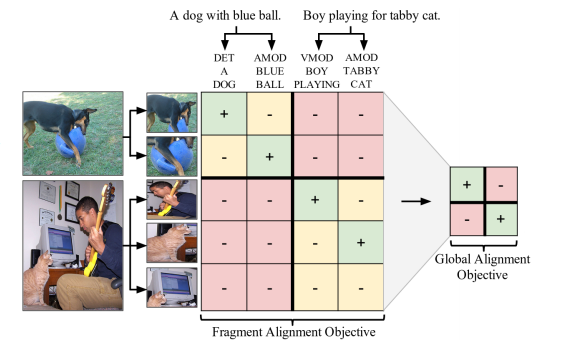
\includegraphics[scale=0.7]{./Imgs/karpathy20014deep_CFG.png}
\caption{دو نمونه از تصاویر و جملات مرتبط با آن‌ها و نتایج  عملکرد اهداف تعریف‌شده روی آن‌ها. سطرها نمایش‌دهنده نواحی مختلف تصویر و ستون‌ها نمایش ‌دهنده قطعه‌های مختلف جملات هستند. سلول‌های قرمز رنگ حالاتی هستند که در آن‌ها $y_{ij} = -1$، سلول‌های زرد نمایش‌دهنده اعضای کیسه‌های مثبت هستند که در آن‌ها $y_{ij} = -1$ است. \cite{karpathy2014deep}}
\label{fig:k2014dCFG}

\end{figure}

\item رتبه‌بندی سراسری

هدف از رتبه‌بندی سراسری این است که شباهت بین یک تصویر و یک جمله، بیشینه شود اگر و تنها اگر تصویر و جمله در واقعیت نیز بیشترین شباهت را به یک‌دیگر داشته باشند. برای این منظور، ابتدا یک امتیاز شباهت بین یک تصویر و یک جمله تعریف می‌شود. این امتیاز مطابق با رابطه\ref{eq:k2014CGS}
تعریف شده و برابر است با میانگین امتیاز شباهت دوبه‌دوی نواحی مختلف تصویر با عبارات مختلف جمله.

\begin{equation}
S_{kl} = \frac{1}{|g_k| (|g_l| + n)} \ML{\Sigma}_{i \in g_k}\ML{\Sigma}_{j\in g_l}max(0,\nu_i^T\cdot s_j)
\label{eq:k2014CGS}
\end{equation}

از آن‌جا که برای دسته‌بندی از روش \lr{mi\_SVM} استفاده می‌شود، تمام امتیازها به صفر محدود می‌شوند. مقدار $n$ که در مخرج کسر اضافه شده است، به صورت تجربی و با آزمون و خطا به‌دست آمده که نتایج را بهبود می‌بخشد. مقدار پیشنهاد شده در پژوهش، $n = 5$ است. تابع کلی هدف سراسری مطابق با رابطه \ref{eq:k2014CG}
تعریف می‌شود.

\begin{equation}
C_G(\Theta) = \ML{\Sigma}_k(
\ML{\Sigma}_l max(0, S_{kl} - S{kk} + \Delta) + 
\ML{\Sigma}_l max(0, S_{lk} - S{kk} + \Delta) 
)
\label{eq:k2014CG}
\end{equation}

در رابطه ارائه شده، $\Delta$ یک ابرپارامتر است که با آزمون و خطا به‌دست می‌آید. عبارت اول درون پرانتز بیان‌کننده امتیاز تصویر و عبارت دوم بیان‌کننده امتیاز جمله هستند.
\end{enumerate}


شکل\ref{fig:k2014res1}
نتایج روش پیشنهاد شده در این پژوهش را ارائه می‌دهد. همان‌طور که در شکل مشخص است، این شبکه قادر به تشخیص اجسام مختلف در تصویر و تولید یک سه‌تایی متناظر هر جسم (ناحیه معنایی) مبتنی بر جملات موجود در مجموعه‌داده مورد استفاده است.

\begin{figure}[H]
\center
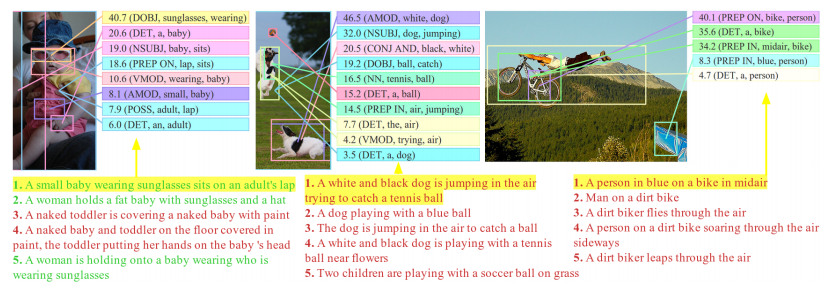
\includegraphics[scale=0.5]{./Imgs/karpathy2014deep_res1.png}
\caption{نتایج نهایی شبکه عصبی ارائه شده. برای هر ناحیه معنایی از تصویر، یک سه‌تایی مبتنی بر جملات موجود در مجموعه‌داده تولید شده است. همین‌طور 5 جمله تولید شده برای هر تصویر به ترتیب امتیاز، درج شده‌اند.\cite{karpathy2014deep}}
\label{fig:k2014res1}
\end{figure}

به علاوه، با توجه به مدل ارائه شده و نگاشت دوطرفه موجود بین تصاویر و جملات، می‌توان با ورودی دادن یک جمله، تصاویر مربوط به آن جمله را استخراج نمود. شکل\ref{fig:k2014res2}
با ثابت در نظر گرفتن جملات، تصاویر مربوط به هر جمله را استخراج و نمایش داده است. هر سطر از این شکل، نمایش‌دهنده تصاویر استخراج شده مرتبط با جمله موجود در آن سطر است.



\begin{figure}[H]
\center
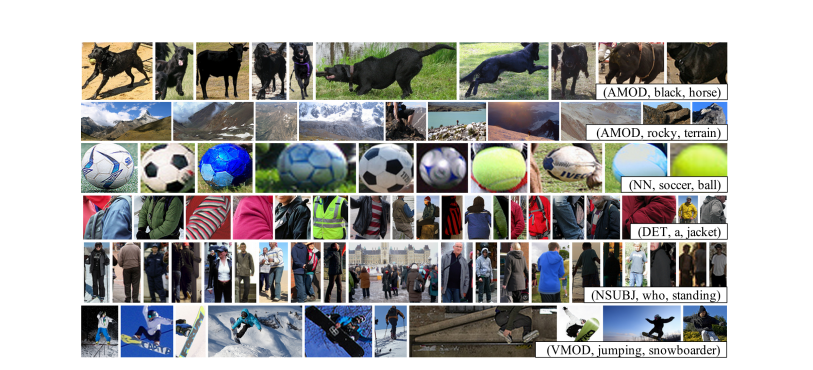
\includegraphics[scale=0.6]{./Imgs/karpathy2014deep_res2.png}
\caption{نتایج حاصل از جستجوی جملات. با ورودی دادن یک جمله، شبکه عصبی ارائه شده در این پژوهش، قادر به استخراج تصاویر مربوط به آن جمله است.\cite{karpathy2014deep}}
\label{fig:k2014res2}
\end{figure}



\subsubsection[هم‌ترازسازی اطلاعات بصری و معنایی به منظور تولید خودکار شرح بر تصاویر]{هم‌ترازسازی\enfootnote{Alignment} اطلاعات بصری و معنایی به منظور تولید خودکار شرح بر تصاویر\cite{Karpathy_2015_CVPR}}
در پژوهش 
\cite{Karpathy_2015_CVPR}
عملیات تولید خودکار شرح برای تصاویر به‌طور کل با استفاده از شبکه‌های عصبی انجام شده‌است. همان‌طور که گفته شد، در این بخش به بررسی درک صحنه در این‌ پژوهش می‌پردازیم.\\
درک صحنه در این پژوهش، با استفاده از به‌کارگیری یک شبکه عصبی کانولوشنی عمیق انجام شده است. این عملیات با انتساب قطعات کوچک جملات به بخش‌های تصویر صورت می‌گیرد. برای این منظور، برای هر قطعه از یک تصویر یک عبارت زبانی توصیف‌کننده قطعه تولید می‌شود. سپس در مرحله دوم با داشتن عبارات توصیف‌کننده قطعات مختلف یک تصویر، عملیات ساخت جمله انجام می‌شود.
\\
ورودی مدل در این قسمت، مجموعه‌ای از تصاویر و شرح تولید شده توسط عوامل انسانی است که در مجموعه‌داده وجود دارد. نکته‌ای که در این بخش حائز اهمیت است، این است که در صورتی‌که یک تصویر به تعدادی از کاربران نمایش داده‌شود و از کاربران خواسته شود که بهترین شرح برای تصویر را بنویسند‌ (بدون این‌که کاربران با یک‌دیگر در ارتباط باشند یا از شرح تولید شده دیگران خبر داشته باشند) بخش‌های یکسانی در شرح‌های تولید شده کاربران وجود خواهد داشت که به نواحی خاصی از تصویر مربوط هستند که موقعیت آن‌ها برای ما نامعلوم است. برای مثال اگر تصویر از یک ریل راه‌آهن و یک قطار باشد، در شرح‌های تولید شده توسط کاربران، عباراتی بیان‌کننده این دو مفهوم وجود خواهند داشت که تکرار آن‌ها در بین شرح‌های موجود از عبارات دیگر بیشتر است. همین موضوع، پایه‌ای برای هم‌ترازسازی در این بخش است. یافتن رابطه مخفی بین عبارات در جملات و نواحی مختلف تصویر منجر به ارائه مدلی برای انتساب این عبارات و نواحی تصویر به یک‌دیگر می‌شود.
\\


\cite{karpathy2014deep}



